\section{CONTEXTUALIZACIÓN}
\subsection{Historia}
\begin{frame}{CONTEXTUALIZACIÓN}
\framesubtitle{Historia y objetivo}
	El objetivo del juego es introducir una bola en hoyos que están distribuidos en el campo con el menor número de golpes. El juego que hoy conocemos fue inventado por los escoceses entre el siglo XIV y el XV \footnote{\bibentry{history}}.
    \begin{figure}[H]
      \centering
      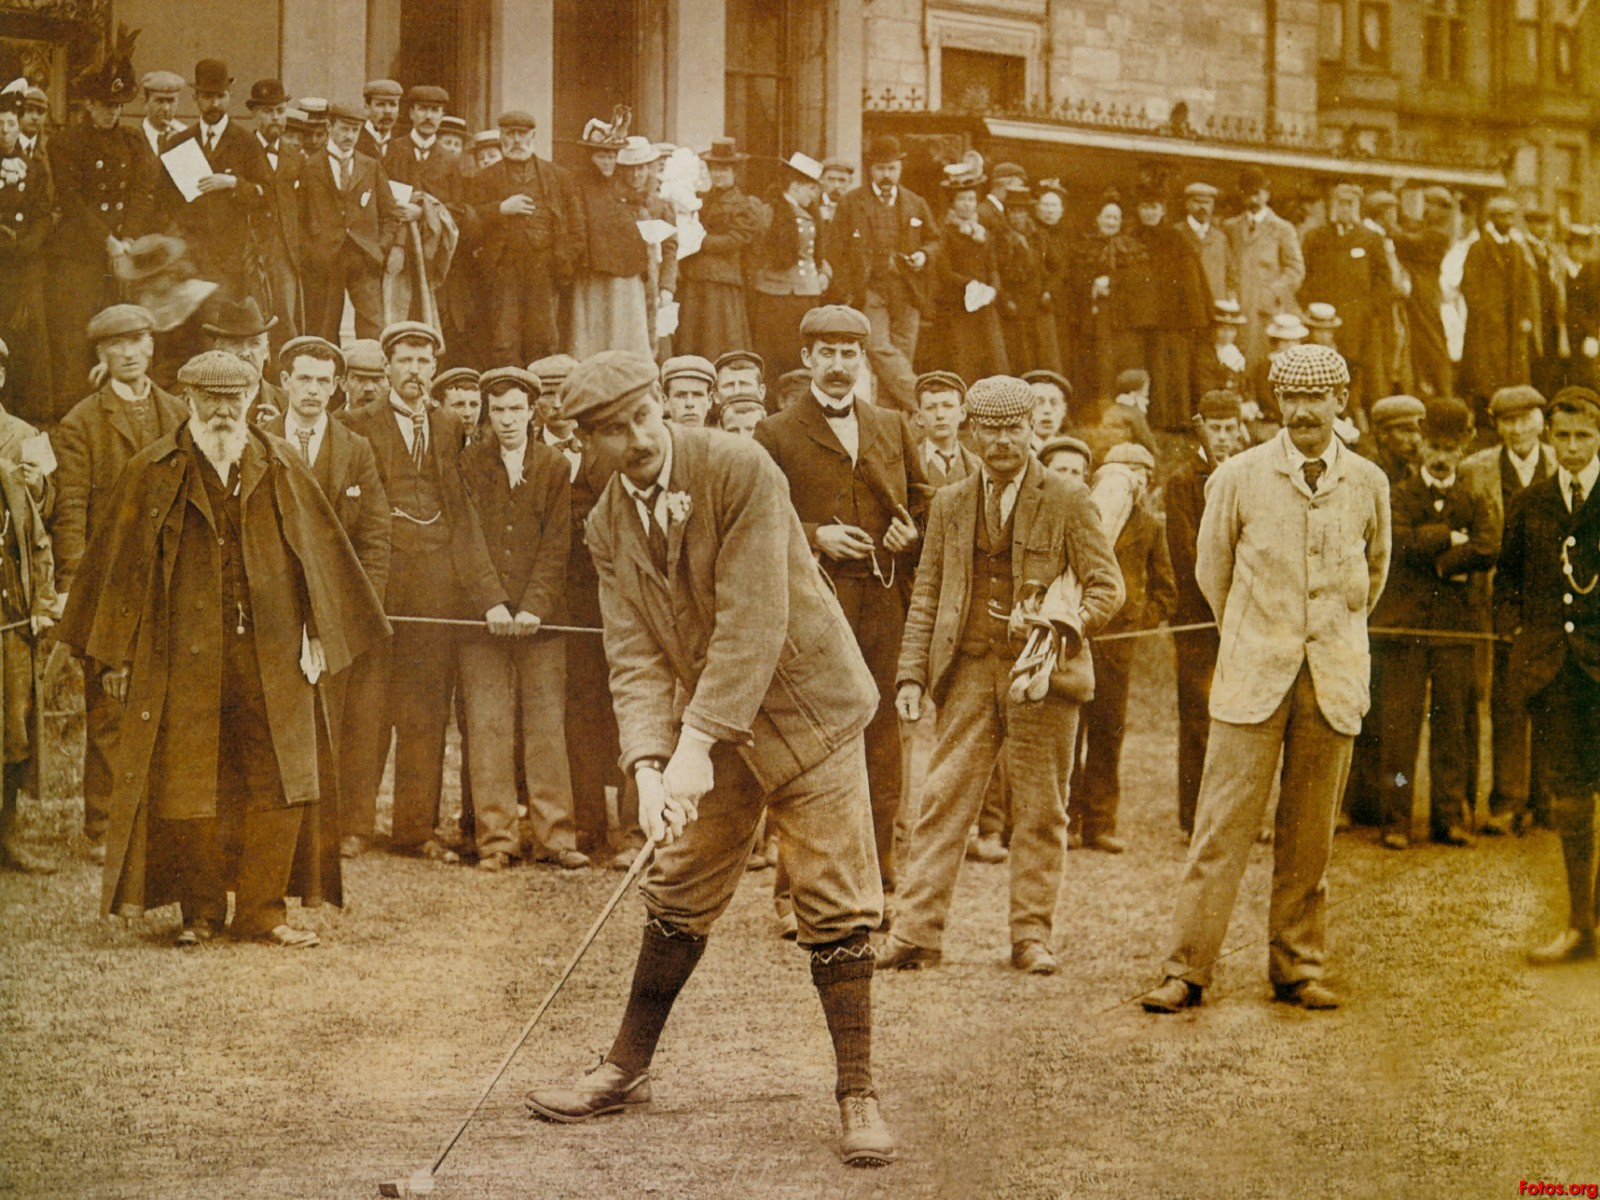
\includegraphics[scale = 0.1]{historia.jpg}
      \caption{Juego de golf, siglo XX\footnotemark{}.}
	\end{figure}
\footnotetext{\bibentry{imgHist}}
\end{frame}
%%%%%%%%%%%%%%%%%%%%%%%%%%%%%%%%%%%%%%%%%
\subsection{Sobre el Campo de Golf}
\begin{frame}{CONTEXTUALIZACIÓN}
\framesubtitle{Sobre el Campo de Golf}
	\begin{figure}[H]
      \centering
      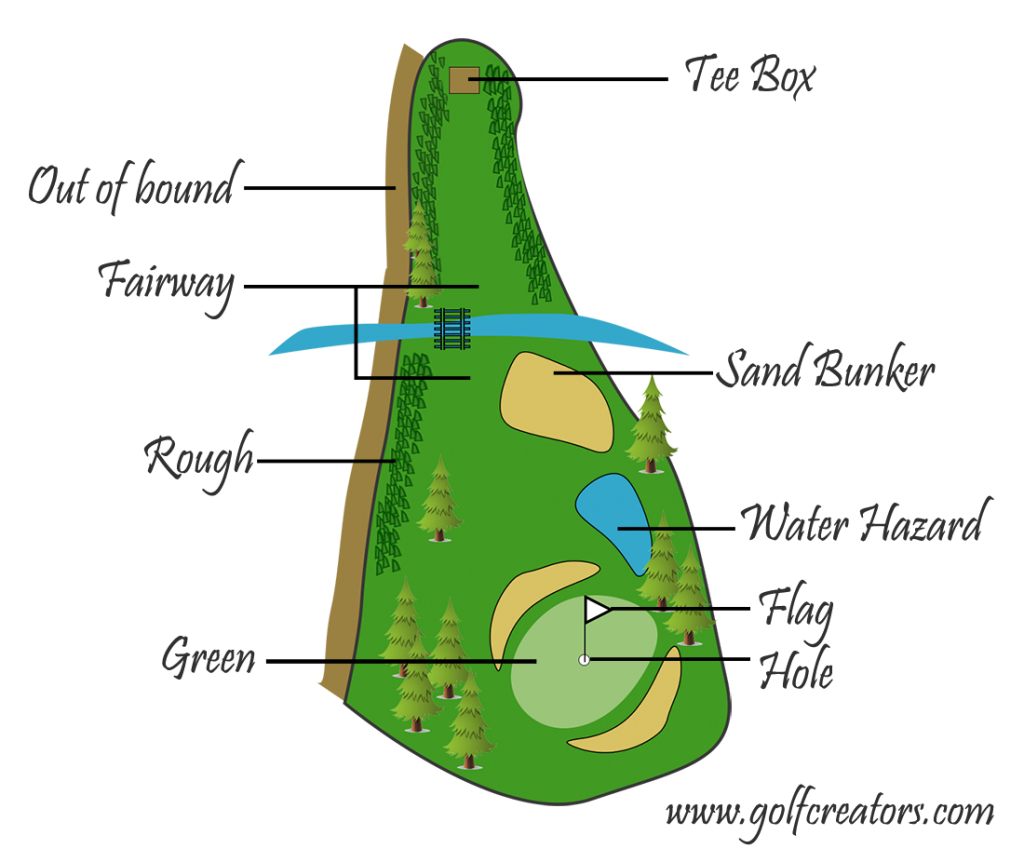
\includegraphics[scale = 0.2]{GolfCourse.png}
      \caption{Campo de Golf.}
	\end{figure}
\end{frame}
%%%%%%%%%%%%%%%%%%%%%%%%%%%%%%%%%%%%%%%
\subsection{Introducción}
\begin{frame}{CONTEXTUALIZACIÓN}
\framesubtitle{Introducción}
¿Cómo cambia el movimiento de un objeto cuando está en un fluido?\\
\url{https://www.khanacademy.org/computing/computer-programming/programming-natural-simulations/programming-forces/a/air-and-fluid-resistance}
\end{frame}


